\documentclass{jlreq}

\usepackage{listings}
\usepackage{caption}
\usepackage{fancyhdr}
\usepackage{graphicx}
\usepackage{mathtools,amssymb}

\lstset{
    language=C, % 使用するプログラム言語を指定
    basicstyle=\ttfamily\footnotesize, % フォントの指定
    numbers=left, % 行番号を表示(必要な場合)
    numberstyle=\tiny, % 行番号のスタイル
    frame=single, % ソースコードを枠で囲む(必要な場合)
    breaklines=true, % 長い行を自動的に折り返す
    captionpos=b, % キャプションの位置を下にする
}
\renewcommand{\lstlistingname}{ソースコード}

\pagestyle{fancy}
\fancyhf{} % 既存のヘッダーとフッターをクリア
\fancyhead[R]{\thepage}% 右上にページ番号を配置
\setlength{\headheight}{17.0pt}
\addtolength{\topmargin}{-7.0pt}

\begin{document}

\tableofcontents
\clearpage

\section{実験機材}

マイコンボードの通し番号:\ 72

使用したパソコン:\ Lenovo Ideapad slim 550(持ち込み)

OS:\ Windows11 Home

\section{理論}

\subsection{PWM}
PWMは,周期一定の矩形波を出力し続けながら,パルス幅を変化させる機能である.
本実験においては,サーボモーターの制御に用いられる.LaunchPadには最大16個のPWM波形を生成する機能があり,
各波形を自由に調整することができる.PWMは2系統存在し,各系統別に4つのPWM生成器を持っている.各生成器は2本の出力ピンを制御することができ,
内蔵RGB LEDを制御するためにはピンの割り当てを適切に行う必要がある.

\subsection{I$^2$C}
I$^2$Cは,低速な周辺機器をマザーボードへ接続するのに用いられる通信規格である.
SCL(クロック)とSDA(データ)の2本の信号線によるシリアル通信であり,この信号線上に複数の機器を接続することができる.
複数の周辺機器は異なるアドレスが付与され,通信の最初にアドレスを指定する.送信と受信は同時に行わず時分割する.
通信速度は遅いため高速に大量のデータをやりとりするような用途には向かないが,
信号線の本数を劇的に削減できるメリットがあるため,速度の要求されない表示パネルなどに利用される.

\subsection{マイコンボード}
本実験で扱うボードは,Tiva C Series LaunchPadのEK-TM4C123GXLというボードである.
このボードには80MHzで動作するプロセッサ,256KBのフラッシュメモリ,32KBのSRAMが搭載されており,各種I/Oを制御することができる.
また,システムクロックには16MHzの水晶発振器を利用している.主な機能はすべて中央のプロセッサに内蔵されており,プロセッサから利用できるピンを
周囲のヘッダに引き出した形になっている.

\subsection{LED}
LaunchPadには3色LEDが内蔵されており,このLEDはGPIOポートFに接続されている.LEDを点灯させるには割り当てられたGPIOピンにH(1)を,
消灯するにはL(0)を出力する.また,PWMの制御によってLEDの光量や色合いを変えられる.

\subsection{ブザー}
圧電ブザーはGPIOピンに接続されており,PWM機能を利用して周期的にON-OFFを繰り返すパルス波形を出力することによって音を鳴らす.
一般的な音階の周波数$f$は次の式で与えられる.
\begin{equation}
  f=440\times2^{\frac{n}{12}}
\end{equation}
$n$の値を$-9$から$+3$と変化させることで音階を表せる.また,ブザーのONとOFFの時間を同じにするためにはパルス幅を周期の半分として与えるなど,
様々な工夫をすることで多種多様な音を表すことができる.

\subsection{LCD}
LCDとはキャラクタ液晶ディスプレイのことである.
LCDを周辺機器として接続し,LCDのアドレスに適切な命令とデータをI$^2$Cバスに流すことでLCDの設定や文字情報を制御することができる.

\section{実験内容}

\subsection{【課題1】仮想シリアルポートへの出力}
プロジェクトblinkyをCCSにインポートした.そして,仮想シリアルポートへの出力をTerminal Pluginによって受信するために,以下のように設定した.
\begin{figure}
  \centering
  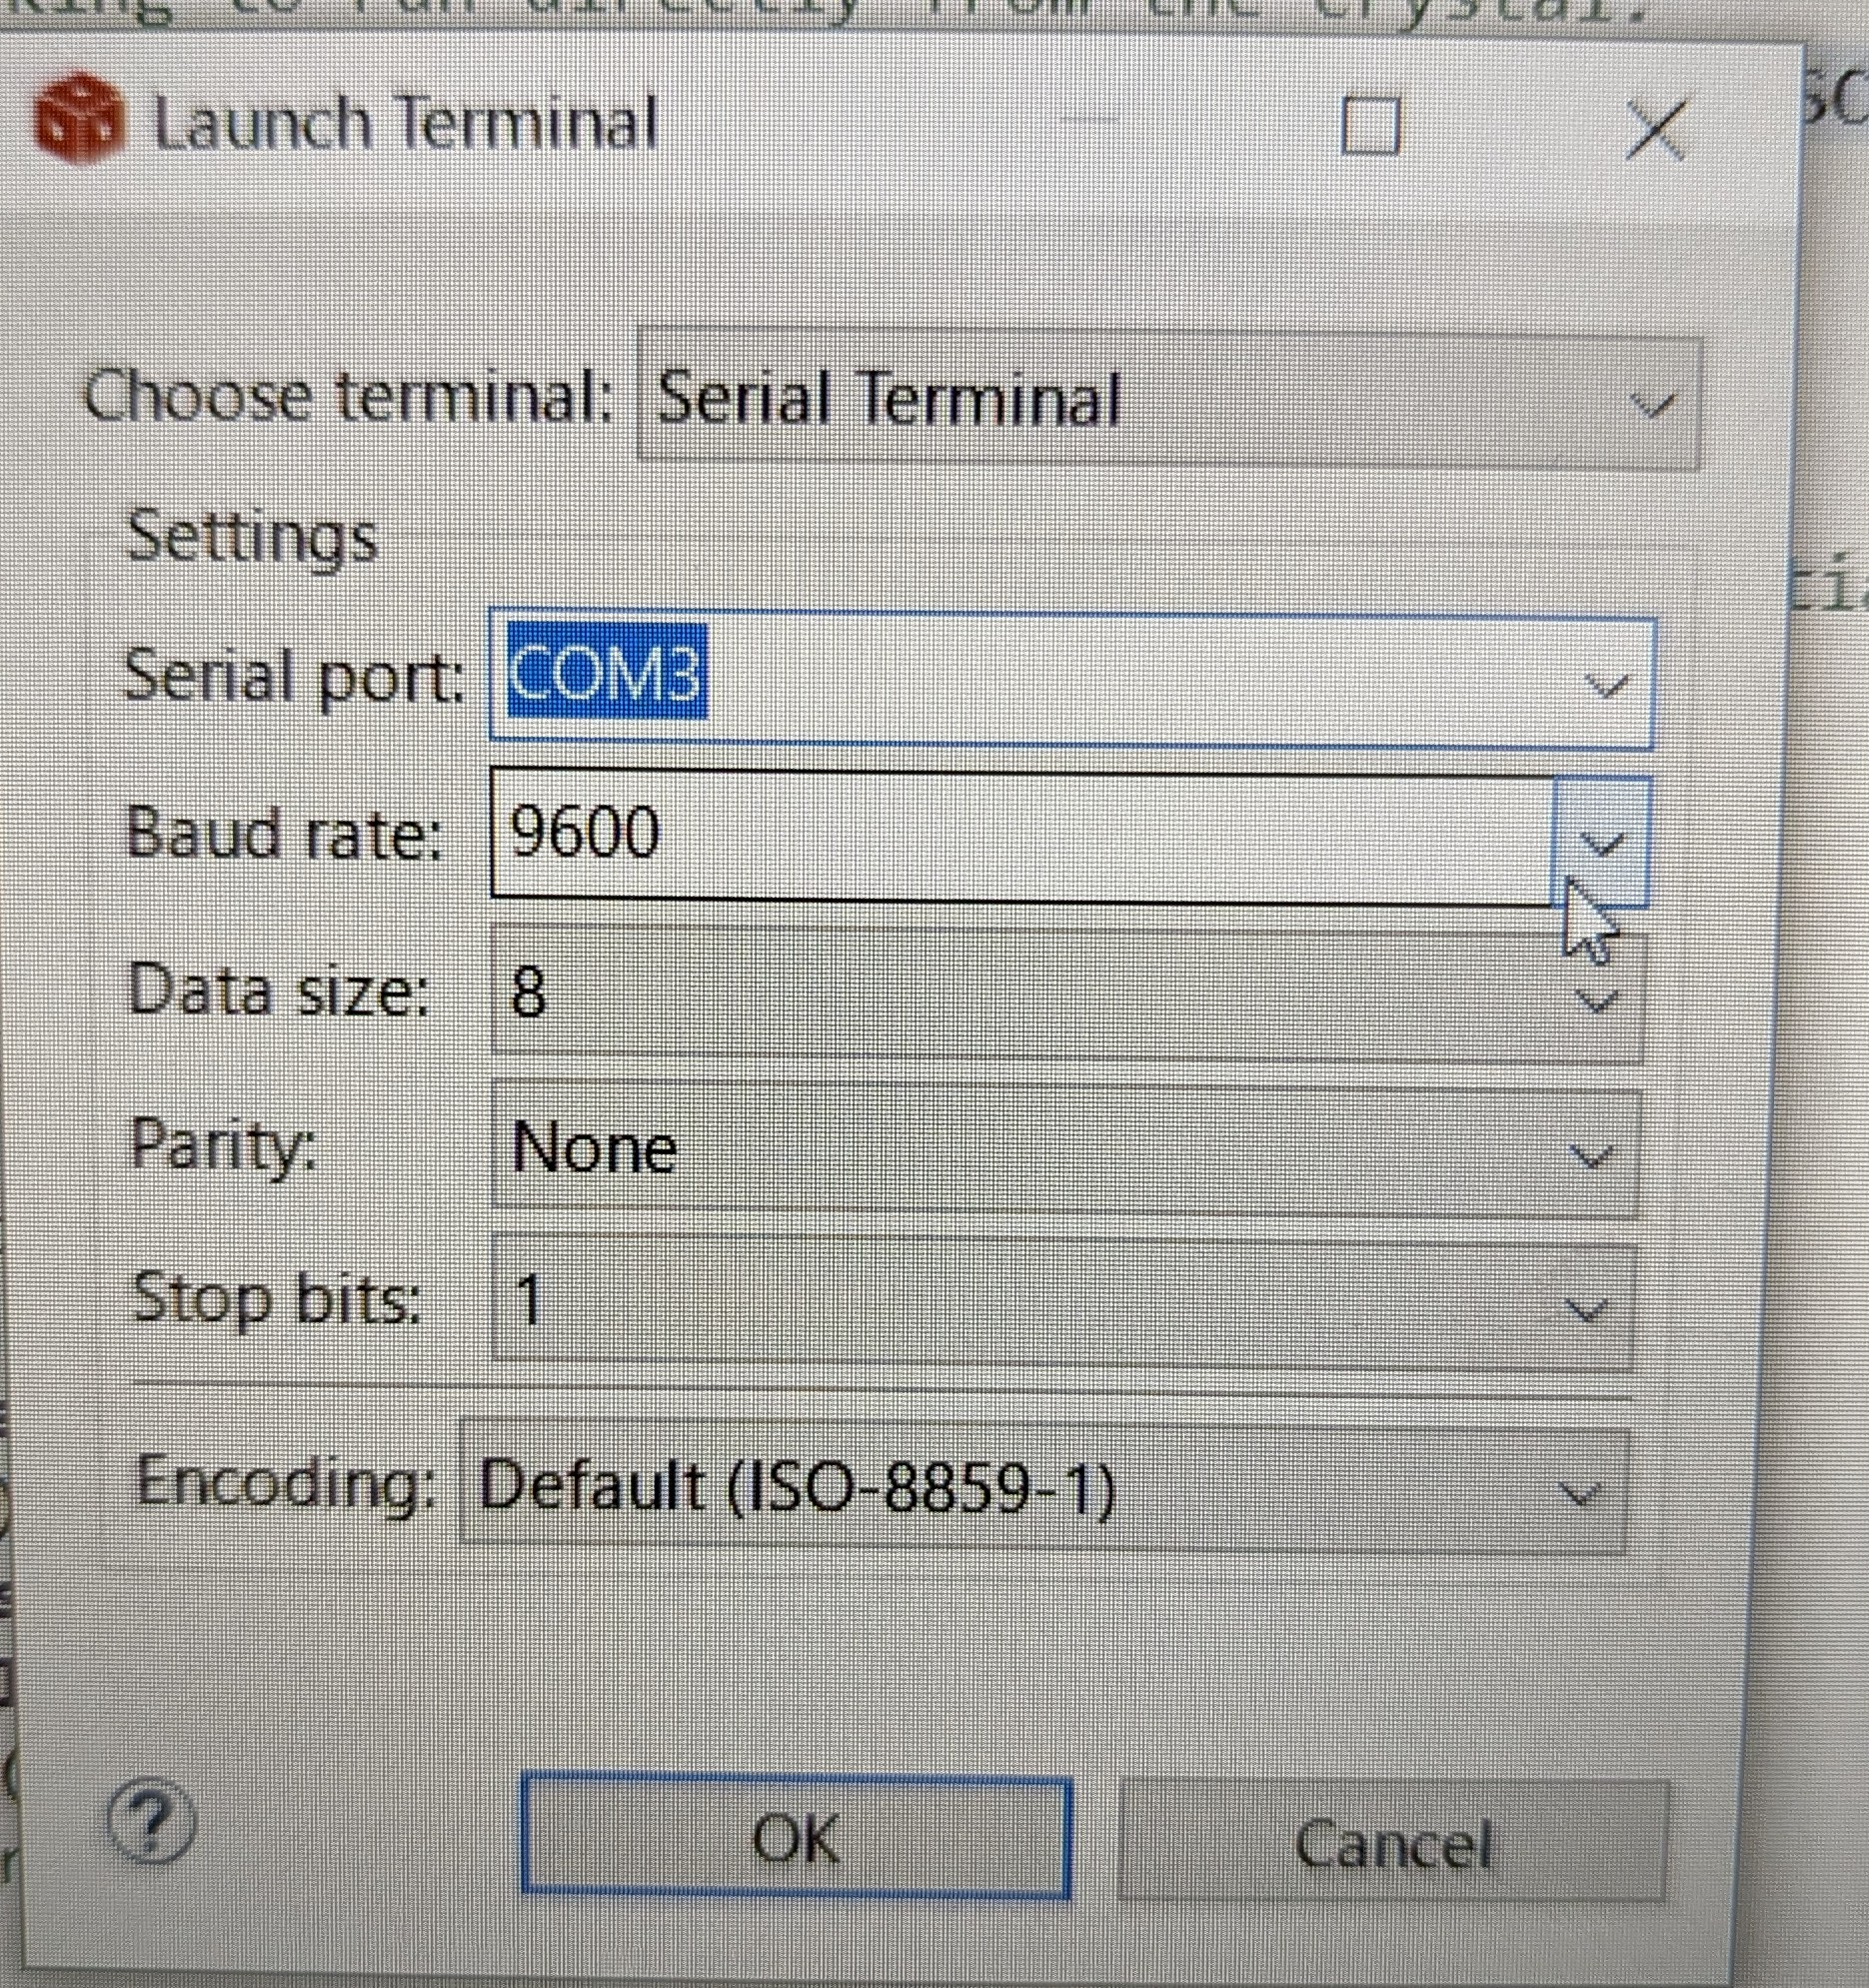
\includegraphics[width=0.3\textwidth]{mysetting.jpg}
  \caption{Terminal Pluginの設定}
  \label{fig:Terminal_Plugin}
\end{figure}

この設定の後,blinky\_main.cのmain()関数内のUARTprintf()のコメントアウトを外してビルドを行い,
仮想シリアルポートへの出力をターミナルを通して確認した.

\subsection{【課題2】blinkyの改造}
blinky\_main.cのmain()関数内でGPIO割り込みを有効化し,initInterruptPins()関数とSW1PinIntHandler()関数を実装し,
SW1の割り込みによってLEDの点灯色を変化させるプログラムに改造した.また,このとき初期状態で有効化されていたSystickの割り込みを無効にした.

\subsection{【課題3】buzzerの改造}
まず,プロジェクトbuzzerをインポートし,未完成のbuzzer.cにおいて音階を表す変数を受け取ってその音を鳴らすtoneBuzzer()関数と,
呼び出すことで音が鳴り止むrestBuzzer()関数を実装した.そして,blinky\_main.cでinitInterruptPins()関数を実装し,
SW1PinIntHandler()関数にてSW1を押すことで音を鳴らしたり消したりするのに加えて,押した回数に従って「ド」から音階を上げて
規定回数以降にまた「ド」に戻るようにプログラムを改造した.

\subsection{【課題4】setAddressLCD()とwriteTextLCD()の実装}
プロジェクトlcdをインポートした後,lcd\_SB1602.cに,LCDの文字位置を指定するsetAddress()関数と,LCDへの文字表示を実行するwriteTextLCD()関数を実装した.
そして,lcd\_main.cで直書きされている文字位置の指定と文字表示の実行のコードをsetAddress()とwriteText()を使うように改造した.

\subsection{【課題5】SW1を押した回数のLCDへの表示}
まず,initInterruptPins()関数を実装し,SW1PinIntHandler()関数を,Systickに割り込みを無効化した後にSW1の押下によって
カウントが実行されてLCDへカウント文字列を表示するように実装した.また,main()関数内でGPIO割り込みを有効化した.

\section{実験結果}

\subsection{【課題1】仮想シリアルポートへの出力}
仮想シリアルポートへの出力を確認するためにターミナルの設定をした後UARTprintf()のコメントアウトを外してビルドを行い実行すると,LEDが青く点滅すると同時に以下のようなメッセージがターミナルで確認できた.

\begin{figure}
  \centering
  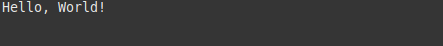
\includegraphics[width=0.9\textwidth]{Hello.png}
  \caption{【課題1】における仮想シリアルポートへの出力内容}
  \label{fig:Hello_World}
\end{figure}

\subsection{【課題2】blinkyの改造}
以下に,blinky\_main.cにおけるinitInterruptPins()のソースコードを示す.

\begin{lstlisting}[label=a2initInt,caption={【課題2】におけるinitInterruptPins関数}]
void initInterruptPins(void) {
    // Clear Interrupt
    GPIOIntClear(GPIO_PORTF_BASE,INT_ALL_BUTTONS);

    // Register a handler function
    GPIOIntRegister(GPIO_PORTF_BASE,SW1PinIntHandler);

    // Set type of interrupt to falling edge
    GPIOIntTypeSet(GPIO_PORTF_BASE,INT_ALL_BUTTONS,GPIO_FALLING_EDGE);
}
\end{lstlisting}

この関数内では,3行目にポートFに接続された全てのスイッチによる割り込みの処理を完了させ,
6行目でポートFにSW1PinIntHandler関数を割り当てて割り込みハンドラを指定し,
9行目でSW1が押されたとき,すなわち波形がL(0)のときに割り込みが発生するように設定した.

次に,blinky\_main.cにおけるSW1PinIntHandler()のソースコードを示す.

\begin{lstlisting}[label=a2SW1Int,caption={【課題2】におけるSW1PinIntHandler関数}]
void SW1PinIntHandler(void) {
    disableSW1PinInt();
    // Clear Interrupt
    clearSW1PinInt();
    SysTickIntDisable();

    GPIOPinWrite(GPIO_PORTF_BASE,base_led_color,0);

    int light[]={LED_BLUE,LED_RED,LED_GREEN,LED_WHITE};
    static int cnt=0;
    base_led_color=light[(++cnt)%4];
    GPIOPinWrite(GPIO_PORTF_BASE,base_led_color,led_color);

    enableSW1PinInt();
}
\end{lstlisting}

この関数内では,2行目に新たなSW1の押下による割り込みを防ぎ,
4行目でSW1による割り込みの処理をクリアし,5行目ではSystickの割り込みを禁止した.
そして,7行目でLEDを一旦消灯させて,9行目から12行目にかけてLEDを点灯させるコードを加えた.初期状態が青でそこから赤,緑,白,青となるように,LEDの色を表すマクロ定数を配列に格納し,
static宣言されたカウント用変数cntの値に応じて色を選択するようにした.
これらの処理を終えたあと,14行目でSW1の押下による新たな割り込みを許可した.

\subsection{【課題3】buzzerの改造}
以下に,toneBuzzer()のソースコードを示す.

\begin{lstlisting}[label=a3toneBuzzer,caption={【課題3】におけるtoneBuzzer関数}]
void toneBuzzer(int tone) {
    PWMGenPeriodSet(PWM0_BASE,PWM_GEN_1,tone);
    PWMPulseWidthSet(PWM0_BASE,PWM_OUT_3,tone>>1);
    PWMOutputState(PWM0_BASE,PWM_OUT_3_BIT,true);
}
\end{lstlisting}

この関数の2行目では出力する波形の周期を与えられた音階toneの周期に設定し,3行目ではパルス幅の設定を行い,4行目でパルス波形の出力を行った.

次に,restBuzzer()のソースコードを示す.

\begin{lstlisting}[label=a3restBuzzer,caption={【課題3】におけるrestBuzzer関数}]
void restBuzzer() {
    PWMOutputState(PWM0_BASE,PWM_OUT_3_BIT,false);
}
\end{lstlisting}

この関数で,PWMOutputState関数の3つ目をbool型のfalseにすることで波形の出力を止めた.

また,buzzer\_main.cにおけるSW1PinIntHandler()を以下に示す.

\begin{lstlisting}[label=a3SW1Int,caption={【課題3】におけるSW1PinIntHandler関数}]
void SW1PinIntHandler(void) {
    GPIOIntDisable(GPIO_PORTF_BASE,INT_ALL_BUTTONS);
    // Clear Interrupt
    GPIOIntClear(GPIO_PORTF_BASE,INT_ALL_BUTTONS);
      
    static int index = 0;
    static bool flag = true;
    int tone_set[] = {O4C, O4D, O4E, O4F, O4G};
      
    if(flag) {
      toneBuzzer(tone_set[index]);
      index = (index + 1) % 5;
    } else {
      restBuzzer();
    }
    
    flag = !flag;
  
    GPIOIntEnable(GPIO_PORTF_BASE,INT_ALL_BUTTONS);
}
\end{lstlisting}

この割り込みハンドラでは,2行目と4行目で新たな割り込みを無効化し,割り込みをクリアした.
また,6行目から17行目にかけてSW1を押した回数によって音を鳴らしたり止めたりすると同時に音階を周期的に変えることを行った.
そして,19行目で新たな割り込みの許可をした.

\subsection{【課題4】setAddressLCD()とwriteTextLCD()の実装}
以下に,setAddressLCD()のソースコードを示す.

\begin{lstlisting}[label=a4setAddress,caption={【課題4】におけるsetAddressLCD関数}]
inline void setAddressLCD(uint8_t x, uint8_t y) {
  uint8_t cursor = x | (y * 0x40);
  uint8_t command[] = {SB1602_COMMAND_SINGLE, 0x80 | cursor};
  writeDataI2C(I2C3_BASE, SB1602_SLAVE_ADDRESS, command, 2);
}
\end{lstlisting}

この関数では,2行目に引数で受け取ったLCDへの表示位置の情報を現在のカーソルとして変数cursorに格納し,
3行目では指定したカーソル位置をコマンドとして送るのに必要な配列command[]に適切な初期化を行い,4行目でI$^2$Cバスを通してLCDにカーソル位置を指定した.

次に,writeTextLCD()のソースコードを示す.

\begin{lstlisting}[label=a4writeText,caption={【課題4】におけるwriteTextLCD関数}]
inline void writeTextLCD(uint8_t *text, uint8_t length) {
  uint8_t command[17];
  command[0] = SB1602_DATA_BURST;
  int i;
  for (i = 0; i < length; i++){
    command[i + 1] = text[i];
  }
  writeDataI2C(I2C3_BASE, SB1602_SLAVE_ADDRESS, command, length + 1);
}
\end{lstlisting}

まず2行目に,送るデータの形式を表すマクロ定数と,引数で与えられた文字列の情報を格納するために要素数を17とした配列command[]を定義した.
3行目から7行目では,先頭にデータを連続的に送ることを意味するマクロ定数を格納し,以降は文字列の長さに応じて文字を格納した.
そして8行目ではI$^2$Cバスを通してLCDに指定したカーソル位置から文字列を表示するコマンドを送った.

\subsection{【課題5】SW1を押した回数のLCDへの表示}
以下に,lcd\_main.cにおけるSW1PinIntHandler()のソースコードを示す.

\begin{lstlisting}[label=a5counter,caption={【課題5】におけるSW1PinIntHandler関数}]
void SW1PinIntHandler(void) {
  SysTickIntDisable();
  disableSW1PinInt();
  clearSW1PinInt();

  static uint8_t spaces[] = {' ', ' ', ' ', ' ', ' ', ' ', ' ', ' ', ' ', ' ', ' ', ' ', ' ', ' ', ' ', ' '};

  setAddressLCD(0, 0);
  writeTextLCD(spaces,16);
  setAddressLCD(0, 1);
  writeTextLCD(spaces,16);

  static uint8_t counter[] = {'0', '0', '0', '0', '0', '0', '0', '0', '0', '0', '0', '0', '0', '0', '0', '0'};
  counter[15]++;

  uint8_t ptr;
  for(ptr = 15; ptr > 0; ptr--){
    if(counter[ptr] > '9') {
      counter[ptr] = '0';
      counter[ptr - 1]++;
    } else break;
  }

  if(counter[ptr] > '9') {
    for(ptr = 0; ptr < 15; ptr++) counter[ptr] = '0';
  }

  uint8_t head = 0;
  while(head < 15 && counter[head] == '0') head++;
  uint8_t counter_length = 16 - head;

  setAddressLCD(head, 0);
  writeTextLCD(&counter[head], counter_length);

  enableSW1PinInt();
}
\end{lstlisting}

この関数では,2行目にSystickによる割り込みを禁止し,3,4行目でSW1による割り込みの禁止とクリアをした.
また,6行目から11行目にかけてLCDへの表示を一旦消し,13行目から33行目にかけてSW1を押した回数の更新とその数のLCDへの表示を行った.
配列counter[]はカウント数を文字列として格納する配列で,表示位置は変数headで指定しsetAddressLCD()とwriteTextLCD()に適切な引数を与えた.
そして,35行目でSW1による割り込みを許可した.

\section{考察}
\paragraph{【考察1】}GPIO割り込みはGPIOポートの電圧の変化を読んで割り込みを認識し,これにより外部からの入力を検知して割り込みを発生させる.
今回の実験では,GPIO割り込みはSW1スイッチの押下による割り込みを発生させる役割を担うと考えられる(外部割り込み).また,Systickは24ビットのダウンカウンタであり,
カウンタが0になると割り込みが発生する.そのため.Systick割り込みはタイマーとしての役割を担うと考えられる(内部割り込み).~\cite{ti}
\paragraph{【考察2】}周辺機器の接続にI$^2$Cを使用すると,機器のmasterとslaveを自由に決めることができる,2本の信号線のみを用いて機器を接続できる,
などの利点がある.~\cite{ti}
\paragraph{【考察3】}割り込みが発生したときだけセンサ読み込みを可能にする実装により,プロセッサのリソースの効率化,割り込みベースによるシステムの単純化,エネルギー効率化などが考えられる.
センサが常に監視状態として働いているとそれだけで電力の消費が大きくなるが,割り込みの採用によりセンサが検知していないときはアイドル状態となり電力の消費を減らすことができる.
また,監視に割いていたリソースをその他の処理に割けるという点でリソースの効率化が見込める.割り込みを用いない場合,センサの処理はポーリング方式などで行う必要があるが,多数のセンサに対応させられるか,
検知した瞬間に反応できるか,といった問題が生じる.その点,割り込みの採用によりこれらの問題の解消が見込める.

\section{問題回答}
\subsection{問題1}
LEDの各色についてOn,Offの2通りを行い,全部消灯している状態は含まないので,求める総数は
\begin{align*}
  2^3-1=7\ 通り
\end{align*}

\subsection{問題2}
問題1におけるOn,Offの2通りから$2^8$通りの制御に変わっただけなので,求める総数は
\begin{align*}
  (2^8)^3-1=16777215\ 通り
\end{align*}

\subsection{問題3}
ソースコード\ref{a3toneBuzzer}を見ると,周期の長さの設定はPWMGenPeriodSet()で行っている.
また,パルス幅はPWMPulseWidthSet()で行っており,3つ目の引数はtone>>1となっているためtoneはパルス波の周期を表していると考えられる.
よって1オクターブ音を高くするには音階の周期を表すマクロ定数(O4C等)を$\frac{1}{2}$倍してtoneBuzzer()に渡すと良い.

\subsection{問題4}
まず,何も抵抗が繋がれていない状態では外部からの静電気などで壊れやすいため抵抗に繋いでおくと不安定を防ぐことができる.
また,プルアップ方式とプルダウン方式のどちらも割り込みによってHIGHとLOWが切り替わるが,プルアップ方式は何もしていないときにHIGHを保ち,
かつ外乱によるノイズなどにも影響されずHIGHを保つ.以上のことから割り込みを受けるピンにおいてプルアップするほうが良い.

\subsection{問題5}
アドレスが$n$ビットで表されるとすると,接続可能な機器は理論上で$2^n$個である.

\subsection{問題6}
\paragraph{delay\_ms()}引数に与えたuint32\_t型の数(マイクロ秒単位)の分だけプログラムを遅らせる
\paragraph{itoh()}uint32\_t型の数値を16進数表記の文字列に変換し,それを格納した配列を返す
\paragraph{itoa()}int32\_t型の数値を10進数表記の文字列に変換し,それを格納した配列を返す

\begin{thebibliography}{9}
  \bibitem{ti}
  Texas Instruments Incorporated.
  \textit{TM4C123GH6PM Microcontroller DATA SHEET}.
  TEXAS INSTRUMENTS.\ 2014.\ https://www.ti.com/lit/ds/spms376e/spms376e.pdf,
  (accsessed 2023-10-31)
\end{thebibliography}

\end{document}